
\documentclass[11pt,a4paper,slovene]{article}

%Uporabljeni paketi
\usepackage[slovene]{babel}
\usepackage[utf8]{inputenc}
\usepackage{lmodern}
\usepackage[T1]{fontenc}
\usepackage{fancyhdr}
\usepackage{caption}
\captionsetup{font={default,footnotesize}, labelfont=bf, format=hang,indention=.0cm}
\usepackage{graphicx,epsfig}
\usepackage{amsmath}
\usepackage{multirow}
\usepackage{color}
\usepackage{url}
\usepackage{makeidx}
\usepackage[official]{eurosym}
\usepackage{float}
\usepackage{changepage}


\usepackage{hyperref}
\hypersetup{
   bookmarksnumbered=true,
   urlbordercolor={0 1 0},
   linkbordercolor={1 1 1},
   unicode=true,
   pdftitle={ Brez\v{z}i\v{c}na in Mobilna Omre\v{z}ja },
   pdfauthor={Asistent},
   pdfdisplaydoctitle=true,
   pdftoolbar=true,
   pdfmenubar=true,
   pdfstartview=X Y Z
}

\urlstyle{same}

\setlength{\parskip}{12pt}
\setlength\parindent{0pt}
\setlength\unitlength{1mm}

\begin{document}
\label{naslov}
\pdfbookmark[1]{Naslov}{naslov}
\thispagestyle{empty}

\begin{center}
\begin{Large}
Brezžična in Mobilna Omrežja\\
Študijsko leto 2022/2023\\
\end{Large}

\vspace*{4cm}
\begin{LARGE}
\textbf{Sobivanje brezžičnih omrežij na istem kanalu\\}
\end{LARGE}
\vspace*{0.5cm}

\begin{Large}
Končno poročilo seminarske naloge\\

\vspace*{4cm}

Jurij Plaskan 63200221, Mojca Kompara 63200147\\
Andraž Sovinec 63200273\\

\vspace*{5cm}
Ljubljana, \today
\end{Large}
\end{center}

\pagebreak
\setcounter{page}{1}
\pagenumbering{arabic}


\label{Kazalo}
\pdfbookmark[1]{Kazalo}{Kazalo}
\tableofcontents
\thispagestyle{empty}
\pagebreak

\section{Uvod}
Programska oprema RaspAP omogoča pretvorbo Raspberry Pi iz navadnega računalnika v dostopno točko osebnega ali lokalnega brezžičnega omrežja. S spreminjanjem nastavitev, se da skonfigurirati RaspAP v dostopno točko lastnega omrežja, ali pa kot dostopno točko v naše domače omrežje. V tej nalogi bomo raziskali zmogljivost omrežnega prenosa omrežja gostujočega na Raspberry Pi, če je več omrežij skonfiguriranih, da tečejo na istem oddajnem kanalu.\\
Sama naloga je precej zanimiva, saj daje vpogled v sobivanje večih brezžičnih omrežij na eni napravi, ter kako to vpliva na zanesljivost in hitrost samega omrežnega prenosa. Poleg tega, pa je bilo za potrebe naloge dodatno raziskati funkcionalnosti RaspAP, ker je močno pripomoglo k splošnemu znanju o delovanju omrežnih dostopnih točk.

\section{Opis uporabljene strojne in programske opreme}
Raspberry Pi je ime serije tako imenovanih \textbf{''Single Board Computer - SBC''}, ki jih razvija Raspberry Pi Foundation (Velika Britanija) v sodelovanju s podjetjem Broadcom. Projekt je bil od začetka usmerjen k poučevanju računalništva v šolah, sedaj pa je eden najbolj prodajanih mikroračunalnikov na svetu in se uporablja za vgrajene računalnike v pametnih hišah, robotiki, monitoring vremena in za stvari kot jih počnemo pri temu predmetu. Raspberry Pi lahko poganja obilico operacijskih sistemov, kot je lastniški Raspberry Pi OS, operacijske siteme, ki temelijo na Linux ali BSD jedru, ter Windows IoT jedro.\cite{enwiki:1146984021}\\
\begin{figure}[H]
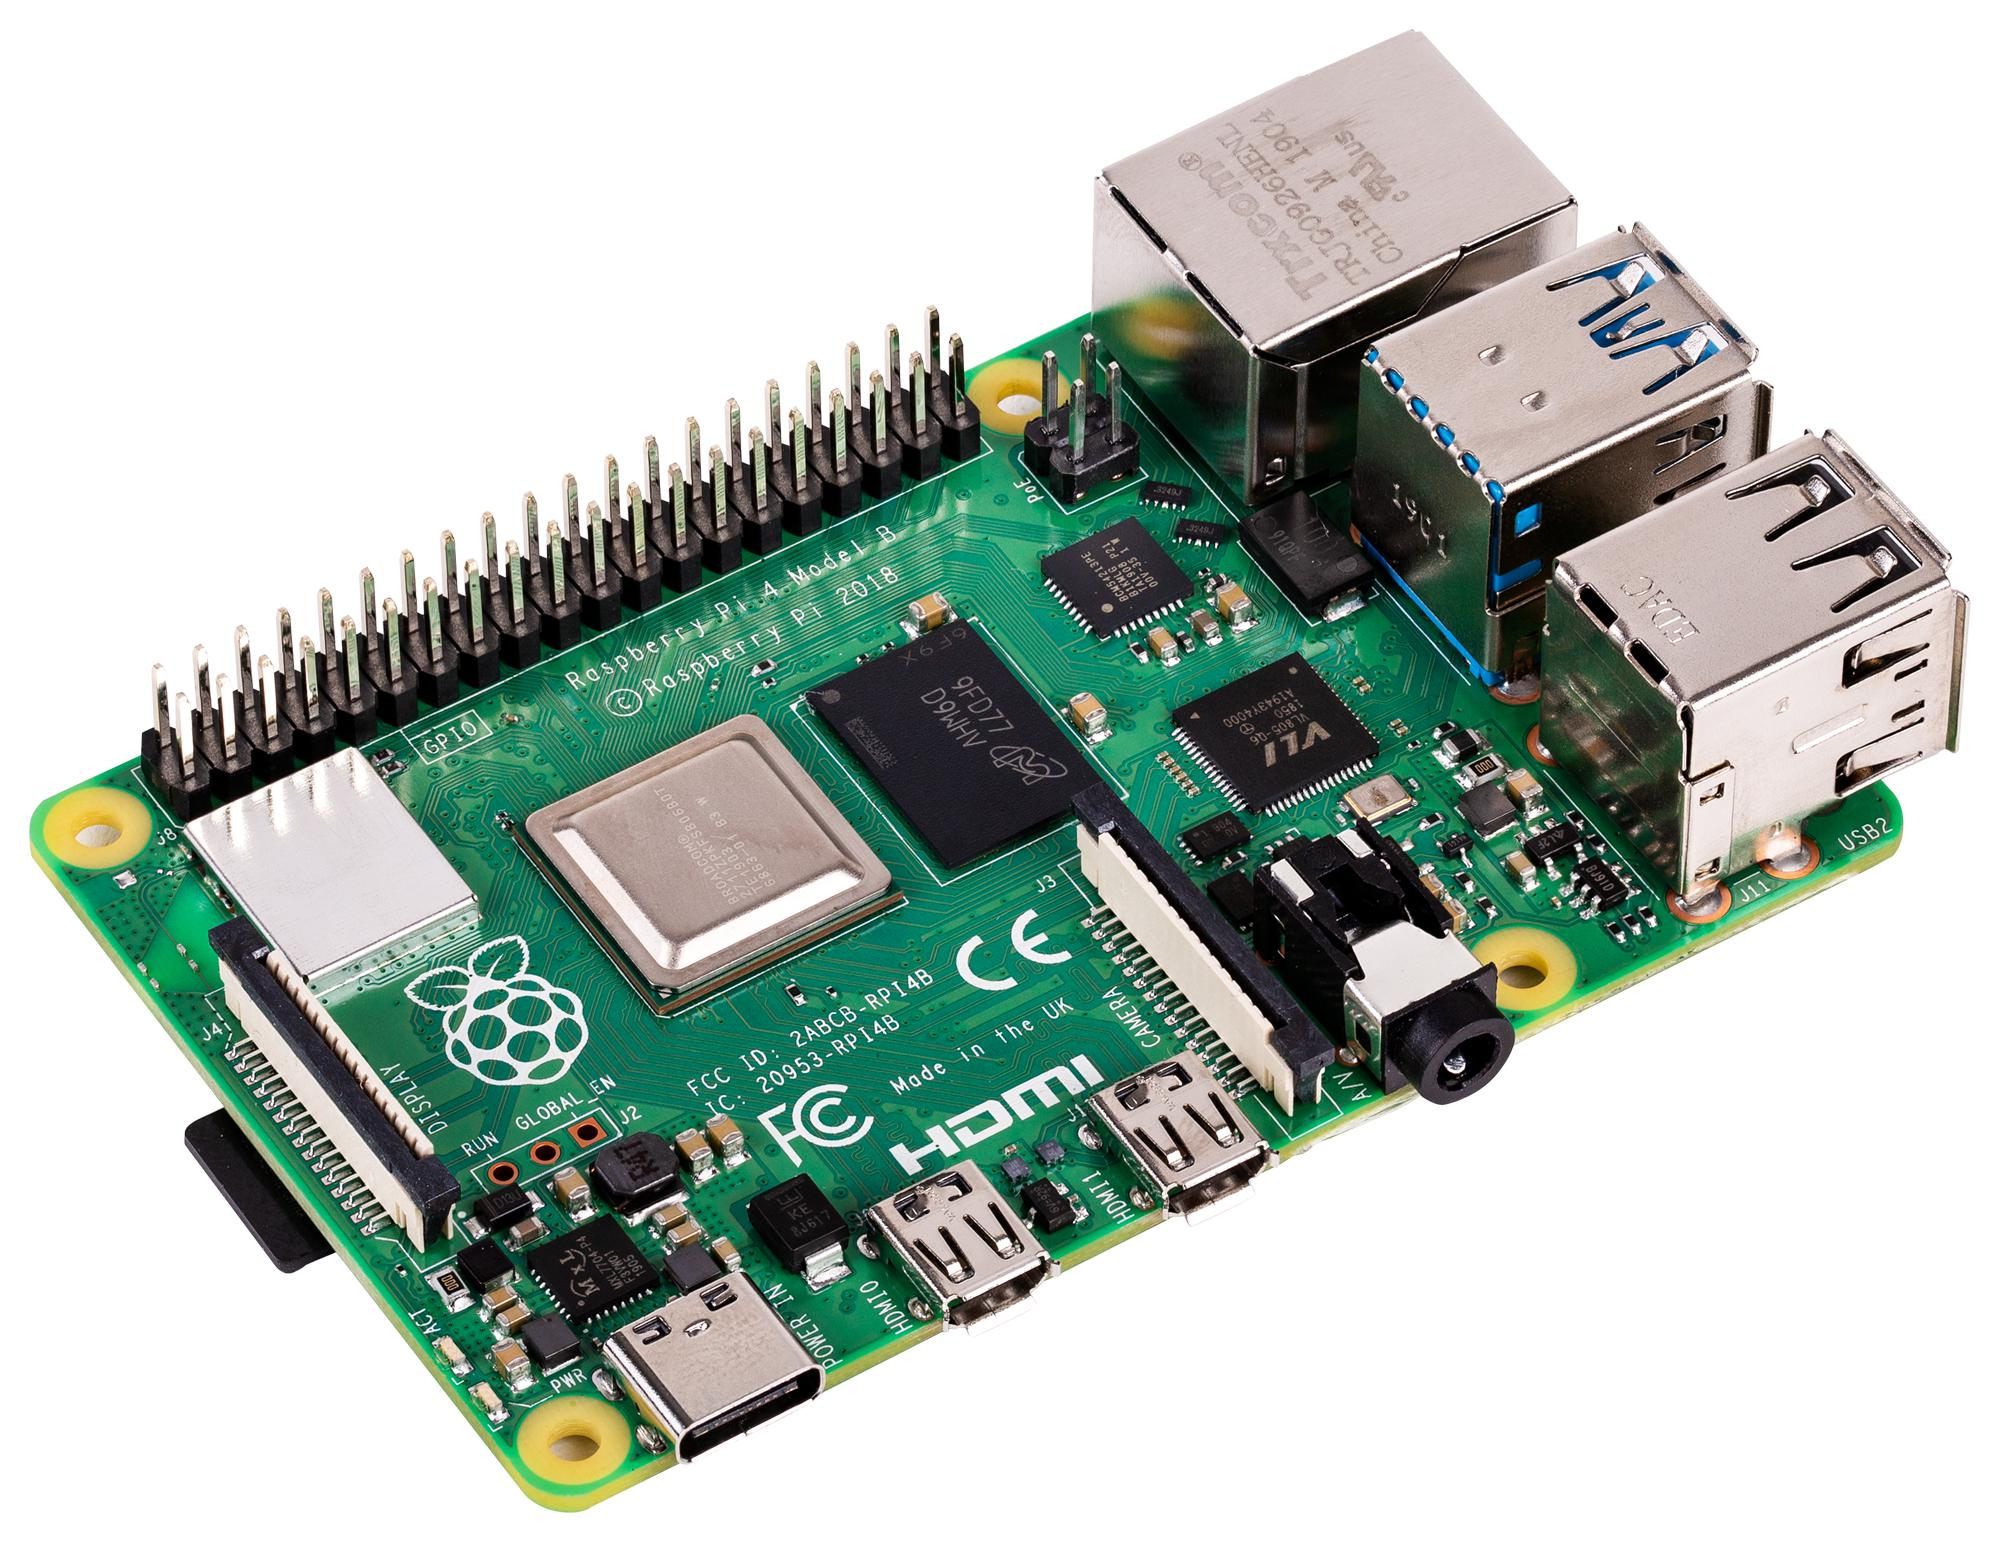
\includegraphics[width=\linewidth]{./rpi4.jpg}
\centering
\caption{Raspberry-Pi 4}
\end{figure}

Za postavitev omrežja in kot dostopno točko smo uporabili Raspberry Pi 4, ki smo ga dobili na vajah pri predmetu, za opravljanje meritev pa kar naše osebne računalnike, da smo lahko zmerili lastnosti omrežnega prenosa pri tem, ko na enem kanalu Raspberry Pi-jevega omrežnega vmesnika teče več omrežij. Brezžična omrežja smo skonfigurirali v programu \textbf{RaspAP}, ki omogoča konfiguracijo Raspberry Pi-jevega brezžičnega vmesnika v dostopno točko omrežja, prav tako pa omogoča nastavitev VPN (Virtual Private Network), Wireguard protokola in še več.\cite{raspap} Za povezovanje na omrežje in tudi kot razširitev števila brezžičnih vmesnikov smo uporabili USB omrežne adapterje D-Link, ki smo jih prav tako dobili na vajah.\\
\begin{figure}[H]
	\includegraphics[width=\linewidth]{./konf\_menu.png}
	\centering
	\caption{Konfiguracijski menu portala RaspAP}
\end{figure}

Zgornja slika prikazuje konfiguracijski portal RaspAP programske opreme - slika je simbolična in ne prikazuje dejanske konfiguracije uporabljenega omrežja.\\

\subsection{CSMA}
Carrier-Sense Multiple Access (CSMA) je protokol za dostop do medija (medium access protocol - MAC) pri katerem vozlišče v omrežju preverja odsotnost preostalega predmeta preden oddaja svoj promet na prenosni medij, ki je bodisi fizično vodilo ali pa elektro-magnetni spekter v primeru Wi-Fi povezave.\\
Oddajnik torej s pomočjo posebnega mehanizma za detekcijo prometa preveri, če je na prenosnem mediju prisoten promet drugega oddajnika. V kolikor zazna, da na mediju poteka prenos drugega oddajnika, počaka dokler se medij ne sprosti in nato ponovno poskusi oddati svoj promet. Tako lahko z uporabo CSMA več vozlišč pošiljajo in prejemajo podatke na istem mediju, kjer je potrebno povedati, da ponavadi ta promet prejmejo vsa ostala vozlišča na mediju, vendar ga obravnava zgolj ciljno vozlišče.\cite{enwiki:1121314888}

CSMA ima dve glavne variacije, ki se tičeta resolucije trkov (CSMA/CA - collision avoidance, CSMA/CD - collision detection) in 4 variacije, ki se tičejo časa pošiljanja na prenosni medij:
\begin{enumerate}
\item 1-persistent: agresivna variacija CSMA algoritma. Če je prenosni medij prost, začne vozlišče takoj oddajati, v kolikor pa ni, pa vozlišče neprestano zaznava ali je prenosni medij prost in nato zopet takoj prične oddajati na medij. V primeru trka pošiljatelj počaka naključno število urinih period in ponovno poskusi isto. Ta variacija je najpogosteje uporabljena v CD sistemih (Ethernet).
\item non-persistent: za razliko od 1-persistent CSMA, ta variacija ne čaka konstantno, da se medij sprosti, temveč takoj preide v fazo naključnega čakanja nekega števila urinih period preden zopet poskusi oddajati na medij. Ta pristop sicer zmanjša možnost pojava trka, vendar ima daljšo začetno zamudo v primerjavi z 1-persistent CSMA.
\item P-persistent: ta je nekakšna kombinacija obeh dveh načinov. V kolikor medij ob prvotnem preverjanju ni prost, konstantno preverja za prostost medija in potem ob ponovno zaznani prostosti medija, poskusi oddati z verjetnostjo \textbf{p}. Če ne odda, počaka na naslednjo prosto časovno rezino, kjer zopet poskusi oddati z verjetnostjo p. V kolikor medij v tistem trenutku ni prost, se ponovi celoten algoritem. Najpogosteje se uporablja v CA sistemih (Wi-Fi).
\item O-persistent: nadzorno vozlišče, vsakemu dodeli mesto v vrstnem redu za pošiljanje. Ko je medij prost, vsako vozlišče čaka, da prejšnje vozlišče preneha oddajati preden poskusi oddajati samo. Prvo vozlišče v vrsti začne oddajati takoj ko je medij prost.
\end{enumerate}

\subsection{Modulacija brezžičnih signalov}
Modulacija je proces spreminjanja ene ali več lastnosti valovne oblike žičnega ali brezžičnega signala, kjer se v bistvu spreminja nosilni signal (carrier signal) z uporabo t.i. modulacijskega signala (modulation signal), ki nosi podatke za prenos. Modulacijski signal je lahko zvočni, video ali digitalni signal (bitstream). Nosilni signal ima po navadi višjo frekvenco kot modulacijski, saj je tako lažje prenašati signal po večjih razdaljah.\\
Pri brezžičnih omrežjih je sicer bolj pomembna plat modulacije, ki se tiče prenašanja večih tokov podatkov skozi en prenosni medij z uporabo "frequency-division multiplexing (FDM)," kjer se pasovna širina prenosnega medija razdeli na neprekrivajoče se frekvenčne pasove, kjer je nato vsak uporabljen za prenos natanko enega toka podatkov. Modulacija se deli na dve vrsti modulacije: analogno in digitalno modulacijo, ki se nato delita dalje, glede na vrsto podatkov, ki se prenašajo in lastnosti signala, ki se spreminja. V radijskih komunikacijah sta najpogostejši AM (amplitudna modulacija) in FM (frekvenčna modulacija).\\
V digitalnih komunikacija poznamo 4 osnovne načine modulacije digitalnega signala, in sicer:
\begin{enumerate}
\item PSK (phase-shift keying)
\item FSK (frequency-shift keying)
\item ASK (amplitude-shidt keying)
\item QAM (quadrature amplitude modulation)\cite{enwiki:1152116503}
\end{enumerate}

Standard 802.11n, ki smo ga uporabili za naša brezžična omrežja uporablja več različnih načinov modulacije, in sicer so najpogostejši načini \textbf{BPSK, QPSK in QAM}. Vsak od teh načinov modulacije se uporablja v standardu z različnimi načini kodiranja (1/2, 3/4, 2/3), ki na koncu odražajo tudi podatkovno hitrost prenosa, merjeno v Mbit/s. Sledeče je slika prvih nekaj modulacijskih shem standarda 802.11n:
\begin{figure}[H]
	\includegraphics[width=\linewidth]{./802\_11.jpg}
	\centering
	\caption{Modulacijske sheme standarda 802.11n}
\end{figure}


\section{Konfiguracija omrežij}
Za začetek je bilo potrebno ugotoviti koliko različnih omrežij je moč skonfigurirati v RaspAP. Tu smo ugotovili v bistvu več stvari. Raspberry Pi ima sam po sebi zgolj en brezžični vmesnik, zaradi česar lahko kot dostopna točka deluje samo za eno konfigurirano omrežje, oz. v hibridnem načinu za dva (eno, ki ga poganjamo, in eno na katerega je RPi povezan kot odjemalec). V odjemalskem načinu pa imaš lahko teoretično skonfiguriranih neskončno omrežij, oziroma toliko kolikor ima Raspberry Pi diskovnega prostora, saj konfiguracija takšnih omrežij poteka v datoteki wpa\_supplicant.conf. To so zgolj privzete možnosti, ki jih ponuja Raspberry Pi, vendar lahko z uporabo zunanjih brezžičnih vmesnikov razširimo število vmesnikov RPi-ja in tako povečamo količino omrežij, ki jim Raspberry Pi lahko deluje kot dostopna točka. Povečevanje števila dostopnih točk na Raspberry Pi sicer nismo uporabili pri sami nalogi, vendar smo poskusili, kako to deluje in je to opisano v razdelku 5.

Omrežje smo postavili na sledeč način. Raspberry Pi-je smo priključili na izposojeno stikalo, tega pa smo nato priključili na sošolčev domač usmerjevalnik, da smo dobili dostop do interneta. Shema topologije je sledeča:
\begin{figure}[H]
	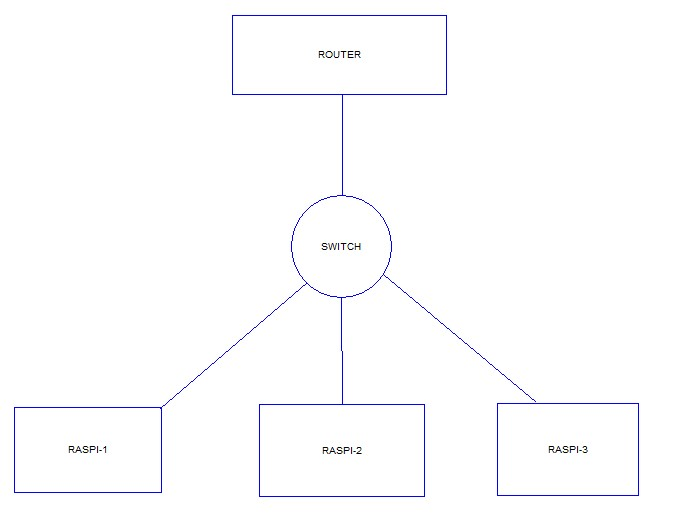
\includegraphics[width=\linewidth]{./topologija.jpg}
	\centering
	\caption{Topologija postavljenega omrežja}
\end{figure}

Ko smo omrežje postavili, smo dostopne točke skonfigurirali tako, da je vsaka svoje omrežje poganjala na kanalu 5 z uporabo standarda 802.11n.

\section{Rezultati}
V tej nalogi smo testirali različne obremenitve omrežnega kanala, in sicer, kadar na istem kanalu tečejo 1, 2 ali pa 3 omrežja. Zajem latence, jitter in delež izgubljenih paketov smo opravili z iperf orodjem in pa kar z ping ukazom, tako za TCP, kot tudi UDP promet. Delež izgubljenih paketov pri TCP prometu je bil skozi testiranje zelo nekonsistenten, saj je pri večih ponovitvah merjenj nihal iz nič na neko popolnoma naključno vrednost. Po pogovoru smo dognali, da je to verjetno zaradi slabše ali zastarele programske opreme, ali pa tudi zaradi zunanjih faktorjev, na katere nismo imeli vpliva. Večinsko je še vedno prevladovalo pri vseh konfiguracijah, da do izgub paketov pri TCP prometu ni prišlo, zatorej je delež pri vseh primerih obravnavan kot 0. Pri UDP prometu pa so izgube datagramov pričakovane, zatorej so navedene.
Za generacijo normalnega prometa smo odprli dva zavihka YouTube, z videi v visoki ločljivosti (torej 1080p 60fps).\\

\subsection{1 omrežje na kanalu}
V tem razdelku so predstavljeni čemur bi lahko rekli kontrolni rezultati, saj je na enem kanalu teklo samo eno omrežje, preostala dva pa vsak na svojem.\\

To je posnetek zaslona vseh omrežij v dometu naših Raspberry Pi-jev, ter tudi kanali na katerih tečejo. Obravnavano omrežje je na 5 kanalu, z imenom \textbf{raspi-21}\\

Kontrolni rezultati so torej kot pričakovani; relativno nizek prenos podatkov in tudi dosti nizka zasedenost pasovne širine. Tu se da pokomentirati to, da je pri TCP prenos podatkov in porabljena pasovna širina v povprečju nižja kot pri standardih 802.11b in 802.11g, ki smo jih potestirali pri drugi domači nalogi pri tem predmetu. To se da pripisati standardu 802.11n, ki je hitrejši kot prej omenjena standarda. UDP prenos pa je vrnil iste rezultate kot pri drugi domači nalogi, torej lahko sklepamo, da standard tu ne naredi bistvene razlike. Delež izgubljenih datagramov je nizek, saj je bilo izgubljenih le 50, kar predstavlja manj kot 1\% vseh poslanih paketov.

Sledeče je še posnetek zaslona ping ukaza, ki prikazuje latenco omrežjo. Tu za komentirati ni pretirano veliko, saj je latenca odvisna od hitrosti pošiljanja in vračanja paketov, ki je redko kdaj konsistentna. Glede na to, da Raspberry Pi ni mišljen kot samostojni usmerjevalnik in zato njegova strojna oprema ni najzmogljivejša, je latenca rahlo višja kot če izvedemo ping ukaz na domači usmerjevalnik (povprečna latenca 2-4ms), vendar so ti rezultati sprejemljivi.\\

\subsection{2 omrežja na istem kanalu}
V tem podrazdelku so prikazani rezultati, kadar na istem kanalu tečeta dva omrežja, tretje pa je na svojem. Sledeča slika zopet prikazuje vsa omrežja v dometu, s tem, da tokrat tečeta na kanalu 5 omrežja \textbf{raspi-21} in \textbf{raspi-23}.\\

Tu so rezultati rahlo bolj zanimiv. Namreč TCP prenos se ni bistveno spremenil (je rahlo nižji), se pa je pomanjšala zasedenost pasovne širine, kar je smiselno saj po standardu omrežje pusti več pasovne širine, da lahko poteka prenos na drugem omrežju kolikor toliko nemoteno.\\

UDP prenos je ostal identičen, se je pa povečalo nihanje latence, ki je skočilo iz $\sim$1ms na kar 5ms. To lahko morda pripišemo konstantni porabi pasovne širine vendar hkratnemu sobivanju dveh omrežij na istem kanalu. Zaradi tega verjetno paketi dalj časa potujejo po omrežjih, da najdejo svoj cilj, saj kot vemo, UDP promet nima preverjanja paketov in se zaradi tega pogosteje "izgubljajo" v omrežju. Delež izgubljenih paketov je v tem primeru narasel na 1,5\% vseh poslanih datagramov.\\

Še ena stvar za povedati pri UDP prometu v tem primeru, je to, da so rezultati tu bili veliko bolj nekonsistentni (prikaz na sledeči sliki), saj je pri eni izmed meritev jitter poskočil na kar 20ms, v še drugem testu pa na kar 36ms. To je lahko zaradi morebitne dodatne zasedenosti omrežja pri poganjanju YouTube posnetkov, zaradi česar so UDP paketi dalj časa potovali proti cilju.

Za konec tega razdelka pa je tu še slika ping ukaza. Tokrat je latenca dosti višja in tudi dosti bolj niha kot pri prvem primeru, kar zopet lahko enostavno pripišemo sobivanju dveh omrežij na enem kanalu.

\subsection{3 omrežja na enem kanalu}
Pri tem primeru smo zopet izmerili iste parametre, na kanalu 5 pa so tokrat tekla vsa 3 omrežja, tore \textbf{raspi-21}, \textbf{raspi-23} in \textbf{raspi-25}. Tokrat TCP prometa ne bomo pokomentirali, saj so rezultati pustili isti učinek kot pri sobivanju dveh omrežij, torej nižji prenos in nižja zasedenost pasovne širine.

Rezultati merjenja UDP prometa z orodjem iperf pa so dali sledeče rezultate:

Iz rezultatov je razvidno, da je prenos in zasedenost pasovne širine ostala enaka, je pa zanimivo to, da se je nihanje latence približno podvojilo, kar pa je (relativno) manjši delež narastka kot pri prehodu iz enega omrežja na kanal, na dva, saj je bil prvi petkratni narastek v latenci, tokrat pa je zgolj dvokraten. Je pa v tem primeru najbolj zanimiv poskok v količini izgubljenih paketov. V prvih dveh primerih se je izgubilo <2\% vseh poslanih paketov, tokrat pa je ta delež narasel na dobrih 3\%, kar je zopet skoraj dvakraten poskok v deležu.\\
Pri ponovitvah testiranju pa je prišlo do sledeče situacije, kjer je nihanje latence zopet naraslo, vendar za manj kot pri prejšnjem primeru, kjer je doseglo celo 20 in 36ms nihanja latence. Ni nam najbolj jasno, zakaj je v tem primeru ob povišanju nihanja latence ta vrednost manjša, zatorej smo si razložili kar kot manjšo zamašitev v omrežnem prenosu. Prav tako pa je narasel delež izgubljenih paketov iz 3.3\% na 4.2\%.\\

Sledeče je še prikaz ping ukaza:

Iz slike je razvidno, da je povprečna latenca zopet narasla, kar je popolnoma pričakovan rezultat, zaradi tega, ne bomo o tem povedali več.
 

\section{Dodatno - Multiple AP konfiguracija}

To smo storili kot poskus, in sicer smo v Raspberry Pi priklopili dva D-Link brezžična adapterja in število brezžičnih vmesnikov tako povečali na 3. Na vsakem od adapterjev je teklo svoje brezžično omrežje, vsako z različnim standardom za brezžično komunikacijo 802.11xx vse pa smo konfigurirali tako da tečejo na kanalu 7.\\
Da smo lahko zagnali nove dostopne točke še na drugih brezžičnih vmesnikih, smo najprej vsak vmesnik posebej skonfigurirali da je poganjal omrežje, hkrati pa smo shranjevali kopije teh konfiguracij v datoteke /etc/hostapd/wlan0.conf - /etc/hostapd/wlan3.conf. Ko smo to naredili, smo naredili kopije in popravili še datoteke /etc/dnsmasq.d/090\_wlan0.conf - /etc/dnsmasq.d/090\_wlan3.conf, tako da je bil notri sledeč zapis:
\begin{verbatim}
	# RaspAP wlan0 configuration
	interface=wlan0
	domain-needed
	dhcp-range=10.3.141.50,10.3.141.254,255.255.255.0,12h
\end{verbatim}
Pri tem je treba poudariti da smo popravili imena vmesnikov in pa ip naslove, kjer smo enastovano inkrementirali drugo številko. Za konec je bilo potrebno še ponovno zagnati dnsmasq.service in ustaviti hostapd.service, nato pa ga ponovno zagnati s komando ''sudo hostapd -dd /etc/hostapd/wlan0.conf /etc/hostapd/wlan1.conf /etc/hostapd/wlan2.conf /etc/hostapd/wlan3.conf.\\
Meritev za takšen način konfiguracije omrežij nismo izvajali, zato se ta razdelek tu konča.

\section{Zaključek}
Rezultati poizkusa so nam dali precejšen vpogled na zmogljivost Rapberry-Pi, če teče več brezžičnih omrežij na istem kanalu. Kot pričakovano se je prenos začel upočasnjevati z večanjem količine omrežij, latenca pa se je hkrati začela višati. Kar se samih nadgradenj tiče, ne vidimo kaj bi lahko v poizkusu izboljšali per se. Lahko bi poskusili meritve opraviti v večih omrežnih topologijah, vendar nimamo zadosti strojne opreme, da bi to bila dosegljiva tarča. Ena izmed možnih sprememb bi bila tudi ta, da bi namesto enotnega standarda uporabili različne standarde za vsako od brezžičnih omrežij, kjer bi eden izmed teh bil tudi standard 802.11ax, kar pa zopet nismo imeli možnosti preizkusiti.\\
Zanimivo bi bilo do konca izpeljati poizkus, ki smo ga na kratko opisali v razdelku 5, vendar na žalost za vse ni časa. Menimo, da bi rezultati prikazali znaten upadec moči omrežij, saj ne verjamemo, da je Raspberry-Pi sposoben brez težav poganjati več brezžičnih omrežij hkrati, a to ne moremo z zagotovostjo trditi.

\section{Tabele rezultatov}


\begin{figure}[H]
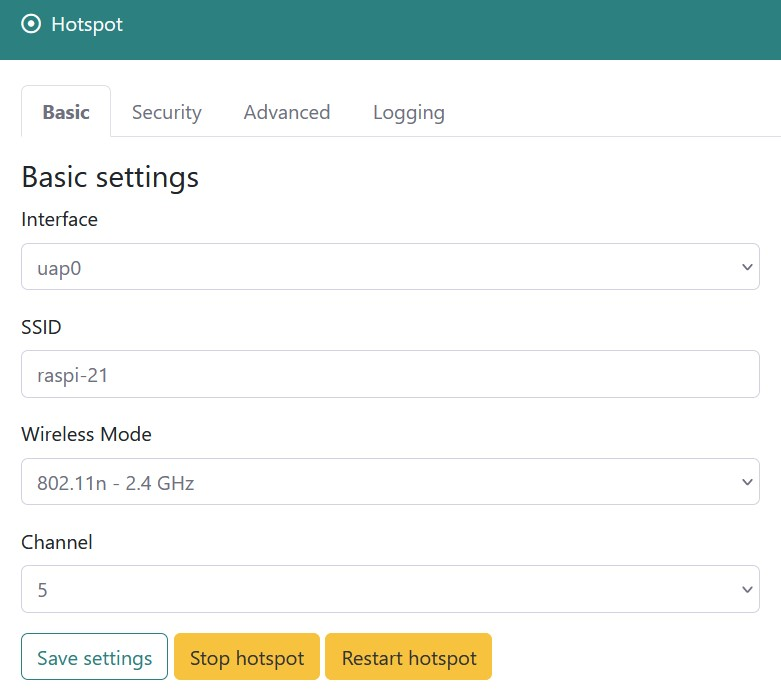
\includegraphics[width=\linewidth]{Conf}
\centering
\caption{Konfiguracija RaspAP za 2.4Gh}
\end{figure}


\begin{figure}[H]
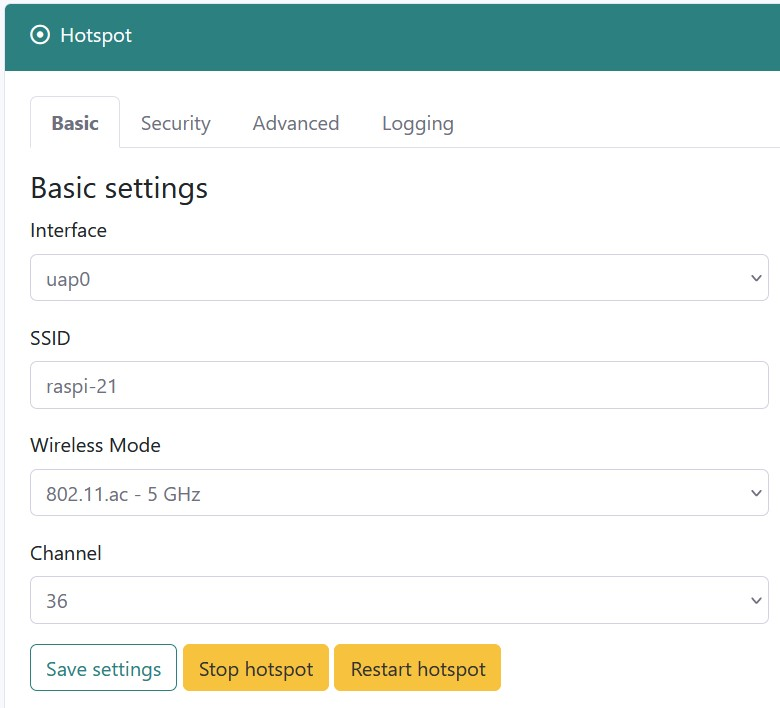
\includegraphics[width=\linewidth]{5GhzConfig}
\centering
\caption{Konfiguracija RaspAP za 5Gh}
\end{figure}

\subsection{Ena naprava - 2.4Gh, iperf}

\begin{table}[H]
	\begin{adjustwidth}{-3cm}{-3cm}
	\centering
		\begin{tabular}{c|c|c|c|c|c}
		\hline
		\textbf{No.} & \textbf{Interval [sec]} & \textbf{Transfer[MBytes]} & \textbf{Bandwidth [Mbits/sec]} & \textbf{Jitter [ms]} & \textbf{Lost/Total} \\
     		\hline
     		1 & 30.0210 & 3.75 & 1.05 & 0.644 & 0\% \\
  		2 & 30.0192 & 3.75 & 1.05 & 1.939 & 0\% \\
  		3 & 30.0183 & 3.75 & 1.05 & 0.661 & 0\% \\
  		4 & 30.0154 & 3.75 & 1.05 & 0.668 & 0\% \\
  		5 & 30.0114 & 3.75 & 1.05 & 1.072 & 0\% \\
  		6 & 29.9944 & 3.75 & 1.05 & 2.960 & 0\% \\
  		7 & 30.0121 & 3.75 & 1.05 & 1.317 & 0\% \\
  		8 & 30.0118 & 3.75 & 1.05 & 0.694 & 0\% \\
  		9 & 30.0121 & 3.75 & 1.05 & 0.738 & 0\% \\
  		10 & 30.0124 & 3.75 & 1.05 & 2.343 & 0\% \\
  		\hline
  		\textbf{Avg} & \textbf{30.0128} & \textbf{3.75} & \textbf{1.05} & \textbf{1.206} & \textbf{0\%} \\
  		\hline
    		\end{tabular}
    	\end{adjustwidth}
\end{table}

\subsection{Dve napravi - 2.4Gh, iperf}
 
 \begin{table}[H]
	\begin{adjustwidth}{-3cm}{-3cm}
	\centering
		\begin{tabular}{c|c|c|c|c|c}
		\hline
		\textbf{No.} & \textbf{Interval [sec]} & \textbf{Transfer[MBytes]} & \textbf{Bandwidth [Mbits/sec]} & \textbf{Jitter [ms]} & \textbf{Lost/Total} \\
     		\hline
     		1 & 30.0118 & 3.75 & 1.05 & 1.954 & 0\% \\
  		2 & 29.6249 & 3.75 & 1.06 & 0.588 & 0\% \\
  		3 & 29.9905 & 3.64 & 1.02 & 1.686 & 3\% \\
  		4 & 30.0776 & 3.64 & 1.02 & 18.773 & 2.9\% \\
  		5 & 30.0270 & 3.73 & 1.04 & 15.664 & 0.6\% \\
  		6 & 30.0243 & 3.60 & 1.01 & 14.052 & 4.2\% \\
  		7 & 30.1309 & 3.75 & 1.05 & 18.353 & 0\% \\
  		8 & 29.9533 & 3.72 & 1.04 & 1.422 & 0.93\% \\
  		9 & 30.0066 & 3.75 & 1.05 & 2.314 & 0\% \\
  		10 & 30.0121 & 3.75 & 1.05 & 1.094 & 0\% \\
  		\hline
  		\textbf{Avg} & \textbf{29.9859} & \textbf{3.71} & \textbf{1.04} & \textbf{7.590} & \textbf{1.16\%} \\
  		\hline
    		\end{tabular}
    	\end{adjustwidth}
\end{table}

\subsection{Tri naprave - 2.4Gh, iperf}
4: 1 datagrams received out-of-order\\
7: WARNING: ack of last datagram failed.\\
 
 \begin{table}[H]
	\begin{adjustwidth}{-3cm}{-3cm}
	\centering
		\begin{tabular}{c|c|c|c|c|c}
		\hline
		\textbf{No.} & \textbf{Interval [sec]} & \textbf{Transfer[MBytes]} & \textbf{Bandwidth [Mbits/sec]} & \textbf{Jitter [ms]} & \textbf{Lost/Total} \\
     		\hline
     		1 & 30.0119 & 3.62 & 1.01 & 13.791 & 3.5\% \\
  		2 & 30.0112 & 3.75 & 1.05 & 7.460 & 0\% \\
  		3 & 30.0314 & 3.69 & 1.03 & 2.044 & 1.7\% \\
  		4 & 29.9184 & 3.75 & 1.05 & 2.476 & 0\% \\
  		5 & 29.9184 & 3.75 & 1.05 & 12.466 & 0\% \\
  		6 & 29.9275 & 3.75 & 1.05 & 3.512 & 0\% \\
  		7 & 30.1465 & 3.62 & 1.01 & 20.326 & 3.6\% \\
  		8 & 30.0751 & 3.73 & 1.04 & 17.111 & 0.63\% \\
  		9 & 30.0187 & 3.74 & 1.04 & 16.161 & 0.41\% \\
  		10 & 30.0119 & 3.75 & 1.05 & 1.289 & 0\% \\
  		\hline
  		\textbf{Avg} & \textbf{30.0071} & \textbf{3.72} & \textbf{1.04} & \textbf{9.664} & \textbf{0.98\%} \\
  		\hline
    		\end{tabular}
    	\end{adjustwidth}
\end{table}

\subsection{Ena naprava - 2.4Gh, ping}

Statistic: 25 packets transmitted, 25 received, 0\% packet loss, time 24053ms
 
 \begin{table}[H]
 	\begin{adjustwidth}{-3cm}{-3cm}
	\centering
		\begin{tabular}{c|c|c}
		\hline
		\textbf{Seq.} & \textbf{Ttl} & \textbf{Time[ms]}\\
     		\hline
     		1 & 128 & 255\\
  		2 & 128 & 5.92\\
  		3 & 128 & 8.74\\
  		4 & 128 & 2.61\\
  		5 & 128 & 25.8\\
  		6 & 128 & 4.39\\
  		7 & 128 & 13.4\\
  		8 & 128 & 4.20\\
  		9 & 128 & 4.35\\
  		10 & 128 & 21.2\\
  		11 & 128 & 4.22\\
  		12 & 128 & 14.9\\
  		13 & 128 & 5.57\\
  		14 & 128 & 4.37\\
  		15 & 128 & 4.12\\
  		16 & 128 & 26.4\\
  		17 & 128 & 2.12\\
  		18 & 128 & 12.0\\
  		19 & 128 & 5.84\\
  		20 & 128 & 19.5\\
  		21 & 128 & 4.16\\
  		22 & 128 & 4.31\\
  		23 & 128 & 29.4\\
  		24 & 128 & 4.19\\
  		25 & 128 & 4.09\\
  		\hline
  		\textbf{Avg} & \textbf{128} & \textbf{19.645}\\
  		\hline
    		\end{tabular}
    	\end{adjustwidth}
\end{table}

\subsection{Dve napravi - 2.4Gh, ping}

Statistic: 20 packets transmitted, 18 received, 10\% packet loss, time 19062ms
 
\begin{table}[H]
	\begin{adjustwidth}{-3cm}{-3cm}
	\centering
		\begin{tabular}{c|c|c}
		\hline
		\textbf{Seq.} & \textbf{Ttl} & \textbf{Time[ms]}\\
     		\hline
     		1 & 128 & 3.69\\
  		2 & 128 & 31.8\\
  		3 & 128 & 59.1\\
  		5 & 128 & 236\\
  		6 & 128 & 11.7\\
  		7 & 128 & 4.44\\
  		8 & 128 & 4.85\\
  		9 & 128 & 4.27\\
  		10 & 128 & 4.76\\
  		11 & 128 & 48.9\\
  		13 & 128 & 96.2\\
  		14 & 128 & 8.05\\
  		15 & 128 & 4.32\\
  		16 & 128 & 4.28\\
  		17 & 128 & 4.40\\
  		18 & 128 & 4.48\\
  		19 & 128 & 15.8\\
  		20 & 128 & 88.8\\
  		\hline
  		\textbf{Avg} & \textbf{128} & \textbf{35.342}\\
  		\hline
    		\end{tabular}
    	\end{adjustwidth}
\end{table}

\subsection{Tri naprave - 2.4Gh, ping}

Statistic: 24 packets transmitted, 20 received, 16.6667\% packet loss, time 23110ms
 
\begin{table}[H]
	\begin{adjustwidth}{-3cm}{-3cm}
	\centering
		\begin{tabular}{c|c|c}
		\hline
		\textbf{Seq.} & \textbf{Ttl} & \textbf{Time[ms]}\\
     		\hline
     		1 & 128 & 2.21\\
  		2 & 128 & 22.2\\
  		3 & 128 & 21.7\\
  		6 & 128 & 308\\
  		7 & 128 & 89.8\\
  		8 & 128 & 4.24\\
  		9 & 128 & 8.54\\
  		10 & 128 & 31.4\\
  		11 & 128 & 2.54\\
  		12 & 128 & 4.11\\
  		13 & 128 & 113\\
  		15 & 128 & 318\\
  		16 & 128 & 6.67\\
  		17 & 128 & 25.8\\
  		18 & 128 & 5.14\\
  		19 & 128 & 4.40\\
  		20 & 128 & 4.44\\
  		21 & 128 & 15.8\\
  		23 & 128 & 132\\
  		24 & 128 & 4.72\\
  		\hline
  		\textbf{Avg} & \textbf{128} & \textbf{56.267}\\
  		\hline
  		\end{tabular}
    	\end{adjustwidth}
\end{table}

\subsection{Ena naprava - 5Gh, iperf}

5, 6, 7, 15: WARNING: ack of last datagram failed.

\begin{table}[H]
	\begin{adjustwidth}{-3cm}{-3cm}
	\centering
		\begin{tabular}{c|c|c|c|c|c}
		\hline
		\textbf{No.} & \textbf{Interval [sec]} & \textbf{Transfer[MBytes]} & \textbf{Bandwidth [Mbits/sec]} & \textbf{Jitter [ms]} & \textbf{Lost/Total} \\
     		\hline
     		1 & 29.9114 & 3.52 & 0.988 & 0.057 & 6.1\% \\
  		2 & 30.0123 & 3.50 & 0.979 & 0.063 & 6.7\% \\
  		3 & 29.9797 & 3.52 & 0.984 & 0.099 & 6.3\% \\
  		4 & 30.0119 & 3.45 & 0.966 & 9.569 & 8\% \\
  		5 & 30.0531 & 3.51 & 0.979 & 18.488 & 6.6\% \\
  		6 & 30.3350 & 3.50 & 0.967 & 17.543 & 6.9\% \\
  		7 & 30.2600 & 3.56 & 0.988 & 21.568 & 5.1\% \\
  		8 & 30.0115 & 3.55 & 0.993 & 0.264 & 5.3\% \\
  		9 & 30.0184 & 3.56 & 0.995 & 11.074 & 5.1\% \\
  		10 & 29.9577 & 3.50 & 0.979 & 0.288 & 6.8\% \\
  		11 & 30.0125 & 3.46 & 0.966 & 7.765 & 7.9\% \\
  		12 & 30.0877 & 3.55 & 0.989 & 11.017 & 5.5\% \\
  		13 & 29.9377 & 3.54 & 0.991 & 0.069 & 5.8\% \\
  		14 & 29.9119 & 3.53 & 0.990 & 0.585 & 6\% \\
  		15 & 30.2956 & 3.53 & 0.977 & 24.393 & 6\% \\
  		\hline
  		\textbf{Avg} & \textbf{30.0531} & \textbf{3.52} & \textbf{0.982} & \textbf{8.123} & \textbf{6.27\%} \\
  		\hline
    		\end{tabular}
    	\end{adjustwidth}
\end{table}

\subsection{Dve napravi - 5Gh, iperf}

3: WARNING: ack of last datagram failed.

\begin{table}[H]
	\begin{adjustwidth}{-3cm}{-3cm}
	\centering
		\begin{tabular}{c|c|c|c|c|c}
		\hline
		\textbf{No.} & \textbf{Interval [sec]} & \textbf{Transfer[MBytes]} & \textbf{Bandwidth [Mbits/sec]} & \textbf{Jitter [ms]} & \textbf{Lost/Total} \\
     		\hline
     		1 & 30.0117 & 3.75 & 1.05 & 10.091 & 0\% \\
  		2 & 30.8304 & 3.01 & 0.82 & 21.039 & 20\% \\
  		3 & 0.0000 & 0.00141 & 0 & 0.000 & 100\% \\
  		4 & 29.6536 & 3.46 & 0.98 & 1.390 & 7.9\% \\
  		5 & 29.3643 & 3.53 & 1.01 & 0.150 & 6\% \\
  		6 & 29.7633 & 3.64 & 1.03 & 0.958 & 3\% \\
  		7 & 30.1383 & 3.74 & 1.04 & 21.099 & 0.45\% \\
  		8 & 29.8519 & 3.58 & 1.01 & 0.142 & 4.7\% \\
  		9 & 29.9635 & 3.72 & 1.04 & 10.233 & 0.82\% \\
  		10 & 30.0116 & 3.75 & 1.05 & 0.241 & 0.11\% \\
  		11 & 30.0166 & 3.47 & 0.97 & 12.601 & 7.5\% \\
  		\hline
  		\textbf{Avg} & \textbf{32.9632} & \textbf{3.24} & \textbf{0.81} & \textbf{7.177} & \textbf{13.68\%} \\
  		\hline
    		\end{tabular}
    	\end{adjustwidth}
\end{table}

\subsection{Ena naprava - 5Gh, ping}

Statistic: 29 packets transmitted, 26 received, 10.3448\% packet loss, time 28104ms
 
\begin{table}[H]
	\begin{adjustwidth}{-3cm}{-3cm}
	\centering
		\begin{tabular}{c|c|c}
		\hline
		\textbf{Seq.} & \textbf{Ttl} & \textbf{Time[ms]}\\
     		\hline
     		1 & 128 & 4.26\\
  		2 & 128 & 4.81\\
  		3 & 128 & 2.65\\
  		4 & 128 & 6.75\\
  		5 & 128 & 3.46\\
  		6 & 128 & 32.6\\
  		7 & 128 & 4.78\\
  		10 & 128 & 202\\
  		11 & 128 & 4.66\\
  		12 & 128 & 3.86\\
  		13 & 128 & 4.69\\
  		14 & 128 & 4.65\\
  		15 & 128 & 41.2\\
  		16 & 128 & 7.21\\
  		17 & 128 & 3.14\\
  		18 & 128 & 207\\
  		19 & 128 & 6.02\\
  		20 & 128 & 5.16\\
  		21 & 128 & 4.58\\
  		22 & 128 & 5.03\\
  		24 & 128 & 29.6\\
  		25 & 128 & 37.8\\
  		26 & 128 & 43.7\\
  		27 & 128 & 5.26\\
  		28 & 128 & 2.41\\
  		29 & 128 & 10.1\\
  		\hline
  		\textbf{Avg} & \textbf{128} & \textbf{26.442}\\
  		\hline
  		\end{tabular}
    	\end{adjustwidth}
\end{table}

\subsection{Dve napravi - 5Gh, ping}

Statistic: 21 packets transmitted, 20 received, 4.7619\% packet loss, time 20041ms
 
 
\begin{table}[H]
	\begin{adjustwidth}{-3cm}{-3cm}
	\centering
		\begin{tabular}{c|c|c}
		\hline
		\textbf{Seq.} & \textbf{Ttl} & \textbf{Time[ms]}\\
     		\hline
     		1 & 128 & 14.3\\
  		2 & 128 & 67.8\\
  		3 & 128 & 71.7\\
  		5 & 128 & 305\\
  		6 & 128 & 217\\
  		7 & 128 & 7.18\\
  		8 & 128 & 7.98\\
  		9 & 128 & 5.03\\
  		10 & 128 & 34.2\\
  		11 & 128 & 529\\
  		12 & 128 & 234\\
  		13 & 128 & 41.9\\
  		14 & 128 & 9.59\\
  		15 & 128 & 7.18\\
  		16 & 128 & 110\\
  		17 & 128 & 223\\
  		18 & 128 & 10.2\\
  		19 & 128 & 65.3\\
  		20 & 128 & 7.85\\
  		21 & 128 & 6.06\\
  		\hline
  		\textbf{Avg} & \textbf{128} & \textbf{98.735}\\
  		\hline
  		\end{tabular}
    	\end{adjustwidth}
\end{table}

\subsection{0 naprav Bluetooth - ping}

Statistic: 19 packets transmitted, 18 received, 5.26316\% packet loss, time 18042ms
 
 
\begin{table}[H]
	\begin{adjustwidth}{-3cm}{-3cm}
	\centering
		\begin{tabular}{c|c|c}
		\hline
		\textbf{Seq.} & \textbf{Ttl} & \textbf{Time[ms]}\\
     		\hline
     		1 & 128 & 2.44\\
  		2 & 128 & 2.81\\
  		3 & 128 & 17.2\\
  		4 & 128 & 17.9\\
  		6 & 128 & 286\\
  		7 & 128 & 2.58\\
  		8 & 128 & 2.36\\
  		9 & 128 & 2.38\\
  		10 & 128 & 2.09\\
  		11 & 128 & 2.13\\
  		12 & 128 & 70.7\\
  		13 & 128 & 2.21\\
  		14 & 128 & 12.2\\
  		15 & 128 & 144\\
  		16 & 128 & 3.97\\
  		17 & 128 & 36.9\\
  		18 & 128 & 2.23\\
  		19 & 128 & 2.19\\
  		\hline
  		\textbf{Avg} & \textbf{128} & \textbf{34.020}\\
  		\hline
  		\end{tabular}
    	\end{adjustwidth}
\end{table}

\subsection{0 naprav Bluetooth - iperf; meritev 1}

\begin{table}[H]
	\begin{adjustwidth}{-3cm}{-3cm}
	\centering
		\begin{tabular}{c|c|c|c}
		\hline
		\textbf{No.} & \textbf{Interval [sec]} & \textbf{Transfer[MBytes]} & \textbf{Bandwidth [Mbits/sec]}\\
     		\hline
     		1 & 0.0000-5.0000 & 0.642 & 1.05\\
  		2 & 5.0000-10.0000 & 0.640 & 1.05\\
  		3 & 10.0000-15.0000 & 0.640 & 1.05\\
  		4 & 15.0000-20.0000 & 0.640 & 1.05\\
  		5 & 20.0000-25.0000 & 0.640 & 1.05\\
  		6 & 25.0000-30.0000 & 0.639 & 1.05\\
  		\hline
  		& 0.0000-30.0131 & 3.75 & 1.05\\
  		\hline
    		\end{tabular}
    	\end{adjustwidth}
\end{table}

Server report (sent 2679 datagrams):\\

\begin{table}[H]
	\begin{adjustwidth}{-3cm}{-3cm}
	\centering
		\begin{tabular}{c|c|c|c|c}
		\hline
		\textbf{Interval [sec]} & \textbf{Transfer[MBytes]} & \textbf{Bandwidth [Mbits/sec]} & \textbf{Jitter [ms]} & \textbf{Lost/Total}\\
     	\hline
     	0.0000-29.8820 & 3.75 & 1.05 & 0.301 & 0\%\\
  		\hline
    		\end{tabular}
    	\end{adjustwidth}
\end{table}

\subsection{0 naprava Bluetooth - iperf; meritev 2}

\begin{table}[H]
	\begin{adjustwidth}{-3cm}{-3cm}
	\centering
		\begin{tabular}{c|c|c|c}
		\hline
		\textbf{No.} & \textbf{Interval [sec]} & \textbf{Transfer[MBytes]} & \textbf{Bandwidth [Mbits/sec]}\\
     		\hline
     		1 & 0.0000-5.0000 & 0.642 & 1.05\\
  		2 & 5.0000-10.0000 & 0.640 & 1.05\\
  		3 & 10.0000-15.0000 & 0.640 & 1.05\\
  		4 & 15.0000-20.0000 & 0.640 & 1.05\\
  		5 & 20.0000-25.0000 & 0.640 & 1.05\\
  		6 & 25.0000-30.0000 & 0.639 & 1.05\\
  		\hline
  		& 0.0000-30.0135 & 3.75 & 1.05\\
  		\hline
    		\end{tabular}
    	\end{adjustwidth}
\end{table}

Server report (sent 2679 datagrams):\\

\begin{table}[H]
	\begin{adjustwidth}{-3cm}{-3cm}
	\centering
		\begin{tabular}{c|c|c|c|c}
		\hline
		\textbf{Interval [sec]} & \textbf{Transfer[MBytes]} & \textbf{Bandwidth [Mbits/sec]} & \textbf{Jitter [ms]} & \textbf{Lost/Total}\\
     	\hline
     	0.0000-30.0121 & 3.75 & 1.05 & 4.907 & 0\%\\
  		\hline
    		\end{tabular}
    	\end{adjustwidth}
\end{table}

\subsection{0 naprava Bluetooth - iperf; meritev 3}

\begin{table}[H]
	\begin{adjustwidth}{-3cm}{-3cm}
	\centering
		\begin{tabular}{c|c|c|c}
		\hline
		\textbf{No.} & \textbf{Interval [sec]} & \textbf{Transfer[MBytes]} & \textbf{Bandwidth [Mbits/sec]}\\
     		\hline
     		1 & 0.0000-5.0000 & 0.642 & 1.05\\
  		2 & 5.0000-10.0000 & 0.640 & 1.05\\
  		3 & 10.0000-15.0000 & 0.640 & 1.05\\
  		4 & 15.0000-20.0000 & 0.640 & 1.05\\
  		5 & 20.0000-25.0000 & 0.640 & 1.05\\
  		6 & 25.0000-30.0000 & 0.639 & 1.05\\
  		\hline
  		& 0.0000-30.0128 & 3.75 & 1.05\\
  		\hline
    		\end{tabular}
    	\end{adjustwidth}
\end{table}

Server report (sent 2679 datagrams):\\

\begin{table}[H]
	\begin{adjustwidth}{-3cm}{-3cm}
	\centering
		\begin{tabular}{c|c|c|c|c}
		\hline
		\textbf{Interval [sec]} & \textbf{Transfer[MBytes]} & \textbf{Bandwidth [Mbits/sec]} & \textbf{Jitter [ms]} & \textbf{Lost/Total}\\
     	\hline
     	0.0000-30.0348 & 3.75 & 1.05 & 1.687 & 0\%\\
  		\hline
    		\end{tabular}
    	\end{adjustwidth}
\end{table}

\subsection{0 naprava Bluetooth - iperf; meritev 4}

\begin{table}[H]
	\begin{adjustwidth}{-3cm}{-3cm}
	\centering
		\begin{tabular}{c|c|c|c}
		\hline
		\textbf{No.} & \textbf{Interval [sec]} & \textbf{Transfer[MBytes]} & \textbf{Bandwidth [Mbits/sec]}\\
     		\hline
     		1 & 0.0000-5.0000 & 0.642 & 1.05\\
  		2 & 5.0000-10.0000 & 0.640 & 1.05\\
  		3 & 10.0000-15.0000 & 0.640 & 1.05\\
  		4 & 15.0000-20.0000 & 0.640 & 1.05\\
  		5 & 20.0000-25.0000 & 0.639 & 1.05\\
  		6 & 25.0000-30.0000 & 0.640 & 1.05\\
  		\hline
  		& 0.0000-30.0137 & 3.75 & 1.05\\
  		\hline
    		\end{tabular}
    	\end{adjustwidth}
\end{table}

Server report (sent 2679 datagrams):\\

\begin{table}[H]
	\begin{adjustwidth}{-3cm}{-3cm}
	\centering
		\begin{tabular}{c|c|c|c|c}
		\hline
		\textbf{Interval [sec]} & \textbf{Transfer[MBytes]} & \textbf{Bandwidth [Mbits/sec]} & \textbf{Jitter [ms]} & \textbf{Lost/Total}\\
     		\hline
     		0.0000-30.0126 & 3.75 & 1.05 & 1.929 & 0\%\\
  		\hline
    		\end{tabular}
    	\end{adjustwidth}
\end{table}

\subsection{0 naprava Bluetooth - iperf; meritev 5}

\begin{table}[H]
	\begin{adjustwidth}{-3cm}{-3cm}
	\centering
		\begin{tabular}{c|c|c|c}
		\hline
		\textbf{No.} & \textbf{Interval [sec]} & \textbf{Transfer[MBytes]} & \textbf{Bandwidth [Mbits/sec]}\\
     		\hline
     		1 & 0.0000-5.0000 & 0.642 & 1.05\\
  		2 & 5.0000-10.0000 & 0.640 & 1.05\\
  		3 & 10.0000-15.0000 & 0.640 & 1.05\\
  		4 & 15.0000-20.0000 & 0.640 & 1.05\\
  		5 & 20.0000-25.0000 & 0.640 & 1.05\\
  		6 & 25.0000-30.0000 & 0.639 & 1.05\\
  		\hline
  		& 0.0000-30.0128 & 3.75 & 1.05\\
  		\hline
    		\end{tabular}
    	\end{adjustwidth}
\end{table}

Server report (sent 2679 datagrams):\\

\begin{table}[H]
	\begin{adjustwidth}{-3cm}{-3cm}
	\centering
		\begin{tabular}{c|c|c|c|c}
		\hline
		\textbf{Interval [sec]} & \textbf{Transfer[MBytes]} & \textbf{Bandwidth [Mbits/sec]} & \textbf{Jitter [ms]} & \textbf{Lost/Total}\\
     		\hline
     		0.0000-30.0181 & 3.75 & 1.05 & 1.636 & 0\%\\
  		\hline
    		\end{tabular}
    	\end{adjustwidth}
\end{table}

\subsection{1 naprava Bluetooth - ping}

Statistic: 23 packets transmitted, 19 received, 17.3913\% packet loss, time 22143
 
 
\begin{table}[H]
	\begin{adjustwidth}{-3cm}{-3cm}
	\centering
		\begin{tabular}{c|c|c}
		\hline
		\textbf{Seq.} & \textbf{Ttl} & \textbf{Time[ms]}\\
     		\hline
     		1 & 128 & 390\\
  		3 & 128 & 203\\
  		4 & 128 & 2.31\\
  		5 & 128 & 6.92\\
  		6 & 128 & 2.36\\
  		7 & 128 & 2.09\\
  		8 & 128 & 2.84\\
  		9 & 128 & 2.76\\
  		10 & 128 & 336\\
  		11 & 128 & 28.7\\
  		12 & 128 & 4.08\\
  		13 & 128 & 3.67\\
  		14 & 128 & 2.91\\
  		15 & 128 & 7.42\\
  		16 & 128 & 3.06\\
  		17 & 128 & 69.3\\
  		21 & 128 & 2.14\\
  		22 & 128 & 9.94\\
  		23 & 128 & 2.21\\
  		\hline
  		\textbf{Avg} & \textbf{128} & \textbf{56.987}\\
  		\hline
  		\end{tabular}
    	\end{adjustwidth}
\end{table}

\subsection{1 naprava Bluetooth - iperf; meritev 1}

\begin{table}[H]
	\begin{adjustwidth}{-3cm}{-3cm}
	\centering
		\begin{tabular}{c|c|c|c}
		\hline
		\textbf{No.} & \textbf{Interval [sec]} & \textbf{Transfer[MBytes]} & \textbf{Bandwidth [Mbits/sec]}\\
     		\hline
     		1 & 0.0000-5.0000 & 0.642 & 1.05\\
  		2 & 5.0000-10.0000 & 0.640 & 1.05\\
  		3 & 10.0000-15.0000 & 0.640 & 1.05\\
  		4 & 15.0000-20.0000 & 0.640 & 1.05\\
  		5 & 20.0000-25.0000 & 0.640 & 1.05\\
  		6 & 25.0000-30.0000 & 0.639 & 1.05\\
  		\hline
  		& 0.0000-30.0124 & 3.75 & 1.05\\
  		\hline
    		\end{tabular}
    	\end{adjustwidth}
\end{table}

Server report (sent 2679 datagrams):\\

\begin{table}[H]
	\begin{adjustwidth}{-3cm}{-3cm}
	\centering
		\begin{tabular}{c|c|c|c|c}
		\hline
		\textbf{Interval [sec]} & \textbf{Transfer[MBytes]} & \textbf{Bandwidth [Mbits/sec]} & \textbf{Jitter [ms]} & \textbf{Lost/Total}\\
     		\hline
     		0.0000-29.9219 & 3.75 & 1.05 & 1.176 & 0\%\\
  		\hline
    		\end{tabular}
    	\end{adjustwidth}
\end{table}

\subsection{1 naprava Bluetooth - iperf; meritev 2}

Kmalu:)\\

\subsection{2 napravi Bluetooth - ping}

Statistic: 18 packets transmitted, 18 received, 0\% packet loss, time 17065
 
\begin{table}[H]
	\begin{adjustwidth}{-3cm}{-3cm}
	\centering
		\begin{tabular}{c|c|c}
		\hline
		\textbf{Seq.} & \textbf{Ttl} & \textbf{Time[ms]}\\
     	\hline
     	1 & 128 & 43.4\\
  		2 & 128 & 1075\\
  		3 & 128 & 45.8\\
  		4 & 128 & 278\\
  		5 & 128 & 2.65\\
  		6 & 128 & 2.73\\
  		7 & 128 & 4.49\\
  		8 & 128 & 8.65\\
  		9 & 128 & 7.33\\
  		10 & 128 & 21.3\\
  		11 & 128 & 4.58\\
  		12 & 128 & 4.84\\
  		13 & 128 & 5.40\\
  		14 & 128 & 4.50\\
  		15 & 128 & 4.74\\
  		16 & 128 & 5.30\\
  		17 & 128 & 4.99\\
  		18 & 128 & 74.1\\
  		\hline
  		\textbf{Avg} & \textbf{128} & \textbf{88.739}\\
  		\hline
  		\end{tabular}
    	\end{adjustwidth}
\end{table}

\subsection{2 napravi Bluetooth - iperf; meritev 1}

\begin{table}[H]
	\begin{adjustwidth}{-3cm}{-3cm}
	\centering
		\begin{tabular}{c|c|c|c}
		\hline
		\textbf{No.} & \textbf{Interval [sec]} & \textbf{Transfer[MBytes]} & \textbf{Bandwidth [Mbits/sec]}\\
     	\hline
     	1 & 0.0000-5.0000 & 0.642 & 1.05\\
  		2 & 5.0000-10.0000 & 0.640 & 1.05\\
  		3 & 10.0000-15.0000 & 0.640 & 1.05\\
  		4 & 15.0000-20.0000 & 0.640 & 1.05\\
  		5 & 20.0000-25.0000 & 0.639 & 1.05\\
  		6 & 25.0000-30.0000 & 0.640 & 1.05\\
  		& 0.0000-30.0128 & 3.75 & 1.05\\
  		\hline
    		\end{tabular}
    	\end{adjustwidth}
\end{table}

Server report (sent 2679 datagrams):\\

\begin{table}[H]
	\begin{adjustwidth}{-3cm}{-3cm}
	\centering
		\begin{tabular}{c|c|c|c|c}
		\hline
		\textbf{Interval [sec]} & \textbf{Transfer[MBytes]} & \textbf{Bandwidth [Mbits/sec]} & \textbf{Jitter [ms]} & \textbf{Lost/Total}\\
     	\hline
     	0.0000-29.8608 & 3.68 & 1.03 & 1.313 & 1.9\%\\
  		\hline
    		\end{tabular}
    	\end{adjustwidth}
\end{table}

\subsection{2 napravi Bluetooth - iperf; meritev 2}

Kmalu:)\\

\subsection{Mikrovalovka Bluetooth - ping}

Statistic: 20 packets transmitted, 20 received, 0\% packet loss, time 19058ms
 
\begin{table}[H]
	\begin{adjustwidth}{-3cm}{-3cm}
	\centering
		\begin{tabular}{c|c|c}
		\hline
		\textbf{Seq.} & \textbf{Ttl} & \textbf{Time[ms]}\\
     	\hline
     	1 & 128 & 30.9\\
  		2 & 128 & 11.0\\
  		3 & 128 & 7.48\\
  		4 & 128 & 4.89\\
  		5 & 128 & 43.0\\
  		6 & 128 & 79.4\\
  		7 & 128 & 96.3\\
  		8 & 128 & 13.0\\
  		9 & 128 & 11.6\\
  		10 & 128 & 4.74\\
  		11 & 128 & 64.2\\
  		12 & 128 & 5.89\\
  		13 & 128 & 4.67\\
  		14 & 128 & 10.9\\
  		15 & 128 & 12.9\\
  		16 & 128 & 11.6\\
  		17 & 128 & 5.28\\
  		18 & 128 & 6.63\\
  		19 & 128 & 4.61\\
  		20 & 128 & 3.58\\
  		\hline
  		\textbf{Avg} & \textbf{128} & \textbf{21.628}\\
  		\hline
  		\end{tabular}
    	\end{adjustwidth}
\end{table}

\subsection{Mikrovalovka Bluetooth - iperf; meritev 1}

\begin{table}[H]
	\begin{adjustwidth}{-3cm}{-3cm}
	\centering
		\begin{tabular}{c|c|c|c}
		\hline
		\textbf{No.} & \textbf{Interval [sec]} & \textbf{Transfer[MBytes]} & \textbf{Bandwidth [Mbits/sec]}\\
     	\hline
     	1 & 0.0000-5.0000 & 0.642 & 1.05\\
  		2 & 5.0000-10.0000 & 0.640 & 1.05\\
  		3 & 10.0000-15.0000 & 0.640 & 1.05\\
  		4 & 15.0000-20.0000 & 0.639 & 1.05\\
  		5 & 20.0000-25.0000 & 0.640 & 1.05\\
  		6 & 25.0000-30.0000 & 0.640 & 1.05\\
  		\hline
  		& 0.0000-30.0126 & 3.75 & 1.05\\
  		\hline
    		\end{tabular}
    	\end{adjustwidth}
\end{table}

Server report (sent 2679 datagrams):\\

\begin{table}[H]
	\begin{adjustwidth}{-3cm}{-3cm}
	\centering
		\begin{tabular}{c|c|c|c|c}
		\hline
		\textbf{Interval [sec]} & \textbf{Transfer[MBytes]} & \textbf{Bandwidth [Mbits/sec]} & \textbf{Jitter [ms]} & \textbf{Lost/Total}\\
     	\hline
     	0.0000-29.8804 & 2.75 & 0.773 & 1.136 & 27\%\\
  		\hline
    		\end{tabular}
    	\end{adjustwidth}
\end{table}

\subsection{Mikrovalovka Bluetooth - iperf; meritev 2}

Kmalu:)\\

\subsection{0 naprav - 5Gh, iperf}

4, 8: WARNING: ack of last datagram failed.

\begin{table}[H]
	\begin{adjustwidth}{-3cm}{-3cm}
	\centering
		\begin{tabular}{l|l|l|l|l|l}
		\hline
		\textbf{No.} & \textbf{Interval [sec]} & \textbf{Transfer[MBytes]} & \textbf{Bandwidth [Mbits/sec]} & \textbf{Jitter [ms]} & \textbf{Lost/Total} \\
     	\hline
     	1 & 30.0167 & 3.71 & 1.04 & 9.762 & 1.1\% \\
  		2 & 29.9436 & 3.70 & 1.04 & 0.037 & 1.5\% \\
  		3 & 30.0114 & 3.60 & 1.01 & 0.164 & 4.1\% \\
  		4 & 30.4505 & 3.48 & 0.959 & 26.947 & 7.3\% \\
  		5 & 30.0045 & 3.48 & 0.974 & 1.979 & 7.2\% \\
  		6 & 30.0116 & 3.53 & 0.986 & 0.062 & 6\% \\
  		7 & 30.0120 & 3.47 & 0.971 & 13.965 & 7.5\% \\
  		8 & 30.1058 & 3.51 & 0.978 & 14.138 & 6.5\% \\
  		9 & 30.0113 & 3.49 & 0.975 & 0.062 & 7.1\% \\
  		\hline
  		\textbf{Avg} & \textbf{30.0630} & \textbf{3.55} & \textbf{1.05} & \textbf{0.993} & \textbf{5.37\%} \\
  		\hline
    		\end{tabular}
    	\end{adjustwidth}
\end{table}

\subsection{1 naprava - 5Gh, iperf}

2: WARNING: ack of last datagram failed.

\begin{table}[H]
	\begin{adjustwidth}{-3cm}{-3cm}
	\centering
		\begin{tabular}{l|l|l|l|l|l}
		\hline
		\textbf{No.} & \textbf{Interval [sec]} & \textbf{Transfer[MBytes]} & \textbf{Bandwidth [Mbits/sec]} & \textbf{Jitter [ms]} & \textbf{Lost/Total} \\
     	\hline
     	1 & 30.0111 & 3.52 & 0.984 & 0.092 & 6.2\% \\
  		2 & 30.1910 & 3.51 & 0.974 & 21.387 & 6.6\% \\
  		3 & 29.9852 & 3.47 & 0.970 & 0.167 & 7.6\% \\
  		4 & 30.0115 & 3.46 & 0.967 & 3.001 & 7.8\% \\
  		5 & 30.0111 & 3.53 & 0.986 & 0.098 & 6.1\% \\
  		6 & 29.9883 & 3.49 & 0.978 & 0.051 & 6.9\% \\
  		7 & 30.0122 & 3.56 & 0.995 & 0.104 & 5.2\% \\
  		8 & 29.9869 & 3.51 & 0.983 & 0.069 & 6.4\% \\
  		9 & 30.0113 & 3.49 & 0.974 & 0.064 & 7.2\% \\
  		10 & 30.0199 & 3.50 & 0.979 & 16.493 & 6.7\% \\
  		11 & 29.9520 & 3.50 & 0.979 & 0.066 & 6.9\% \\
  		12 & 30.0126 & 3.51 & 0.982 & 0.076 & 6.4\% \\
  		13 & 30.0120 & 3.56 & 0.994 & 0.044 & 5.2\% \\
  		\hline
  		\textbf{Avg} & \textbf{30.0158} & \textbf{3.51} & \textbf{1.05} & \textbf{3.209} & \textbf{6.55\%} \\
  		\hline
    		\end{tabular}
    	\end{adjustwidth}
\end{table}

\subsection{2 napravi - 5Gh, iperf}

3, 8: WARNING: ack of last datagram failed.

\begin{table}[H]
	\begin{adjustwidth}{-3cm}{-3cm}
	\centering
		\begin{tabular}{l|l|l|l|l|l}
		\hline
		\textbf{No.} & \textbf{Interval [sec]} & \textbf{Transfer[MBytes]} & \textbf{Bandwidth [Mbits/sec]} & \textbf{Jitter [ms]} & \textbf{Lost/Total} \\
     	\hline
     	1 & 30.0629 & 3.48 & 0.970 & 0.060 & 7.4\% \\
  		2 & 29.7333 & 3.49 & 0.984 & 0.324 & 7.1\% \\
  		3 & 30.0682 & 3.54 & 0.988 & 16.294 & 5.7\% \\
  		4 & 30.0207 & 3.56 & 0.995 & 8.601 & 5.2\% \\
  		5 & 30.0025 & 3.54 & 0.990 & 0.045 & 5.7\% \\
  		6 & 29.5966 & 3.53 & 1.000 & 0.042 & 6\% \\
  		7 & 30.0143 & 3.48 & 0.971 & 0.469 & 7.4\% \\
  		8 & 30.0147 & 3.51 & 0.981 & 0.077 & 6.5\% \\
  		9 & 30.0135 & 3.54 & 0.990 & 0.058 & 5.6\% \\
  		\hline
  		\textbf{Avg} & \textbf{29.9474} & \textbf{3.52} & \textbf{0.985} & \textbf{2.8856} & \textbf{6.29\%} \\
  		\hline
    		\end{tabular}
    	\end{adjustwidth}
\end{table}

\subsection{0 naprav Bluetooth - 5G, ping}

Statistic: 20 packets transmitted, 16 received, 20\% packet loss, time 19100ms
 
 
\begin{table}[H]
	\begin{adjustwidth}{-3cm}{-3cm}
	\centering
		\begin{tabular}{c|c|c}
		\hline
		\textbf{Seq.} & \textbf{Ttl} & \textbf{Time[ms]}\\
     	\hline
     	1 & 128 & 2.79\\
  		2 & 128 & 2.87\\
  		3 & 128 & 4.12\\
  		4 & 128 & 2.53\\
  		5 & 128 & 2.34\\
  		6 & 128 & 2.29\\
  		7 & 128 & 21.2\\
  		9 & 128 & 424\\
  		12 & 128 & 204\\
  		13 & 128 & 2.87\\
  		14 & 128 & 2.49\\
  		15 & 128 & 2.12\\
  		16 & 128 & 2.61\\
  		18 & 128 & 380\\
  		19 & 128 & 60.2\\
  		20 & 128 & 65.8\\
  		\hline
  		\textbf{Avg} & \textbf{128} & \textbf{73.915}\\
  		\hline
  		\end{tabular}
    	\end{adjustwidth}
\end{table}


\subsection{1 naprava Bluetooth - 5G, ping}

Statistic: 24 packets transmitted, 20 received, 16.6667\% packet loss, time 23119ms
 
 
\begin{table}[H]
	\begin{adjustwidth}{-3cm}{-3cm}
	\centering
		\begin{tabular}{c|c|c}
		\hline
		\textbf{Seq.} & \textbf{Ttl} & \textbf{Time[ms]}\\
     	\hline
     	1 & 128 & 2.19\\
  		2 & 128 & 2.56\\
  		3 & 128 & 2.85\\
  		4 & 128 & 1.87\\
  		5 & 128 & 2.24\\
  		9 & 128 & 304\\
  		10 & 128 & 2.62\\
  		11 & 128 & 2.87\\
  		12 & 128 & 2.43\\
  		13 & 128 & 2.26\\
  		14 & 128 & 2.36\\
  		15 & 128 & 51.6\\
  		17 & 128 & 304\\
  		18 & 128 & 2.80\\
  		19 & 128 & 2.58\\
  		20 & 128 & 2.33\\
  		21 & 128 & 1.83\\
  		22 & 128 & 88.1\\
  		23 & 128 & 20.4\\
  		24 & 128 & 32.5\\
  		\hline
  		\textbf{Avg} & \textbf{128} & \textbf{41.745}\\
  		\hline
  		\end{tabular}
    	\end{adjustwidth}
\end{table}

\subsection{2 napravi Bluetooth - 5G, ping}

Statistic: 21 packets transmitted, 18 received, 14.2857\% packet loss, time 20092ms
 
 
\begin{table}[H]
	\begin{adjustwidth}{-3cm}{-3cm}
	\centering
		\begin{tabular}{c|c|c}
		\hline
		\textbf{Seq.} & \textbf{Ttl} & \textbf{Time[ms]}\\
     	\hline
     	1 & 128 & 12.1\\
  		2 & 128 & 2.25\\
  		3 & 128 & 2.77\\
  		4 & 128 & 2.62\\
  		5 & 128 & 2.31\\
  		6 & 128 & 2.73\\
  		7 & 128 & 2.38\\
  		8 & 128 & 2.30\\
  		9 & 128 & 2.13\\
  		10 & 128 & 12.1\\
  		11 & 128 & 2.32\\
  		12 & 128 & 2.78\\
  		13 & 128 & 2.78\\
  		14 & 128 & 2.51\\
  		16 & 128 & 305\\
  		19 & 128 & 203\\
  		20 & 128 & 2.38\\
  		21 & 128 & 2.83\\
  		\hline
  		\textbf{Avg} & \textbf{128} & \textbf{31.519}\\
  		\hline
  		\end{tabular}
    	\end{adjustwidth}
\end{table}



\subsection{Mikrovalovka - 5Gh, iperf}

\begin{table}[H]
	\begin{adjustwidth}{-3cm}{-3cm}
	\centering
		\begin{tabular}{l|l|l|l|l|l}
		\hline
		\textbf{No.} & \textbf{Interval [sec]} & \textbf{Transfer[MBytes]} & \textbf{Bandwidth [Mbits/sec]} & \textbf{Jitter [ms]} & \textbf{Lost/Total} \\
     	\hline
     	1 & 30.0116 & 3.54 & 0.989 & 0.047 & 5.7\% \\
  		2 & 29.9334 & 3.60 & 1.01 & 1.024 & 4\% \\
  		3 & 30.0113 & 3.52 & 0.983 & 0.198 & 6.3\% \\
  		4 & 30.0108 & 3.53 & 0.986 & 0.139 & 6\% \\
  		5 & 29.6757 & 3.46 & 0.979 & 0.152 & 7.7\% \\
  		\hline
  		\textbf{Avg} & \textbf{29.9474} & \textbf{3.52} & \textbf{0.985} & \textbf{2.8856} & \textbf{6.29\%} \\
  		\hline
    		\end{tabular}
    	\end{adjustwidth}
\end{table}

\subsection{Mikrovalovka - 5Gh, ping}

Statistic: 23 packets transmitted, 19 received, 17.3913\% packet loss, time 22085ms
 
 
\begin{table}[H]
	\begin{adjustwidth}{-3cm}{-3cm}
	\centering
		\begin{tabular}{c|c|c}
		\hline
		\textbf{Seq.} & \textbf{Ttl} & \textbf{Time[ms]}\\
     	\hline
     	3 & 128 & 2.86\\
  		4 & 128 & 2.75\\
  		5 & 128 & 2.45\\
  		6 & 128 & 2.26\\
  		7 & 128 & 2.97\\
  		8 & 128 & 2.68\\
  		9 & 128 & 39.3\\
  		10 & 128 & 47.4\\
  		12 & 128 & 304\\
  		13 & 128 & 2.39\\
  		14 & 128 & 2.82\\
  		15 & 128 & 2.36\\
  		16 & 128 & 2.93\\
  		17 & 128 & 31.9\\
  		18 & 128 & 31.8\\
  		19 & 128 & 382\\
  		21 & 128 & 203\\
  		22 & 128 & 2.71\\
  		23 & 128 & 2.35\\
  		\hline
  		\textbf{Avg} & \textbf{128} & \textbf{56.362}\\
  		\hline
  		\end{tabular}
    	\end{adjustwidth}
\end{table}

\pagebreak
\bibliographystyle{plain}
\bibliography{references}

\end{document}











